\section{Cải tiến mô hình}
\subsection{Phân tích độ khó dữ liệu trước huấn luyện}
\label{subsec:pretrain_data_analysis}

Trước giai đoạn huấn luyện mô hình, phân tích định lượng được thực hiện để đánh giá mức độ khó nội tại của bài toán phân đoạn nguyên liệu thực phẩm. So với các tập semantic segmentation tổng quát, FoodSeg103 có đặc trưng fine-grained rõ rệt: nhiều lớp nguyên liệu có màu sắc và texture gần nhau, ranh giới giữa các vùng thường mờ, đồng thời nhiều thành phần xuất hiện chồng lấp trong cùng một ảnh. Các yếu tố này làm mô hình nhẹ như BiSeNet dễ mất chi tiết cục bộ trong quá trình downsampling, đặc biệt tại vùng biên và các lớp có diện tích nhỏ. FoodSeg103 cũng là benchmark ingredient-level gồm 103 lớp nguyên liệu, nơi thành phần có thể chồng lấp, biến đổi mạnh theo cách chế biến và có độ tương đồng thị giác cao.

Để lượng hóa độ khó, các chỉ số phân tích tiền huấn luyện gồm: độ nghiêm trọng ở mức ảnh, độ nghiêm trọng ở mức lớp, quan hệ giữa pixel accuracy và present-class mIoU, các lớp đóng vai trò ``sink class'', và ma trận nhầm lẫn giữa các lớp. Các phân tích này không nhằm kết luận hiệu năng mô hình cuối cùng, mà nhằm chỉ ra sớm các kiểu lỗi có xác suất cao khi huấn luyện mô hình lightweight trên dữ liệu thực phẩm fine-grained.

\subsubsection{Phân bố độ nghiêm trọng ở mức ảnh}

Hình~\ref{fig:image_severity_distribution} biểu diễn phân bố điểm độ nghiêm trọng của ảnh. Phần lớn ảnh tập trung trong khoảng điểm cao, đặc biệt từ khoảng $0.75$ đến $0.95$, với mật độ lớn nhất gần vùng $0.88$--$0.92$. Kết quả này cho thấy đa số mẫu trong tập dữ liệu không thuộc nhóm dễ, mà chứa nhiều yếu tố gây nhiễu cho phân đoạn như nhiều nguyên liệu đồng thời, ranh giới yếu, vùng giao nhau phức tạp hoặc texture khó phân biệt.

\begin{figure}[H]
    \centering
    \begin{subfigure}{0.49\linewidth}
        \centering
        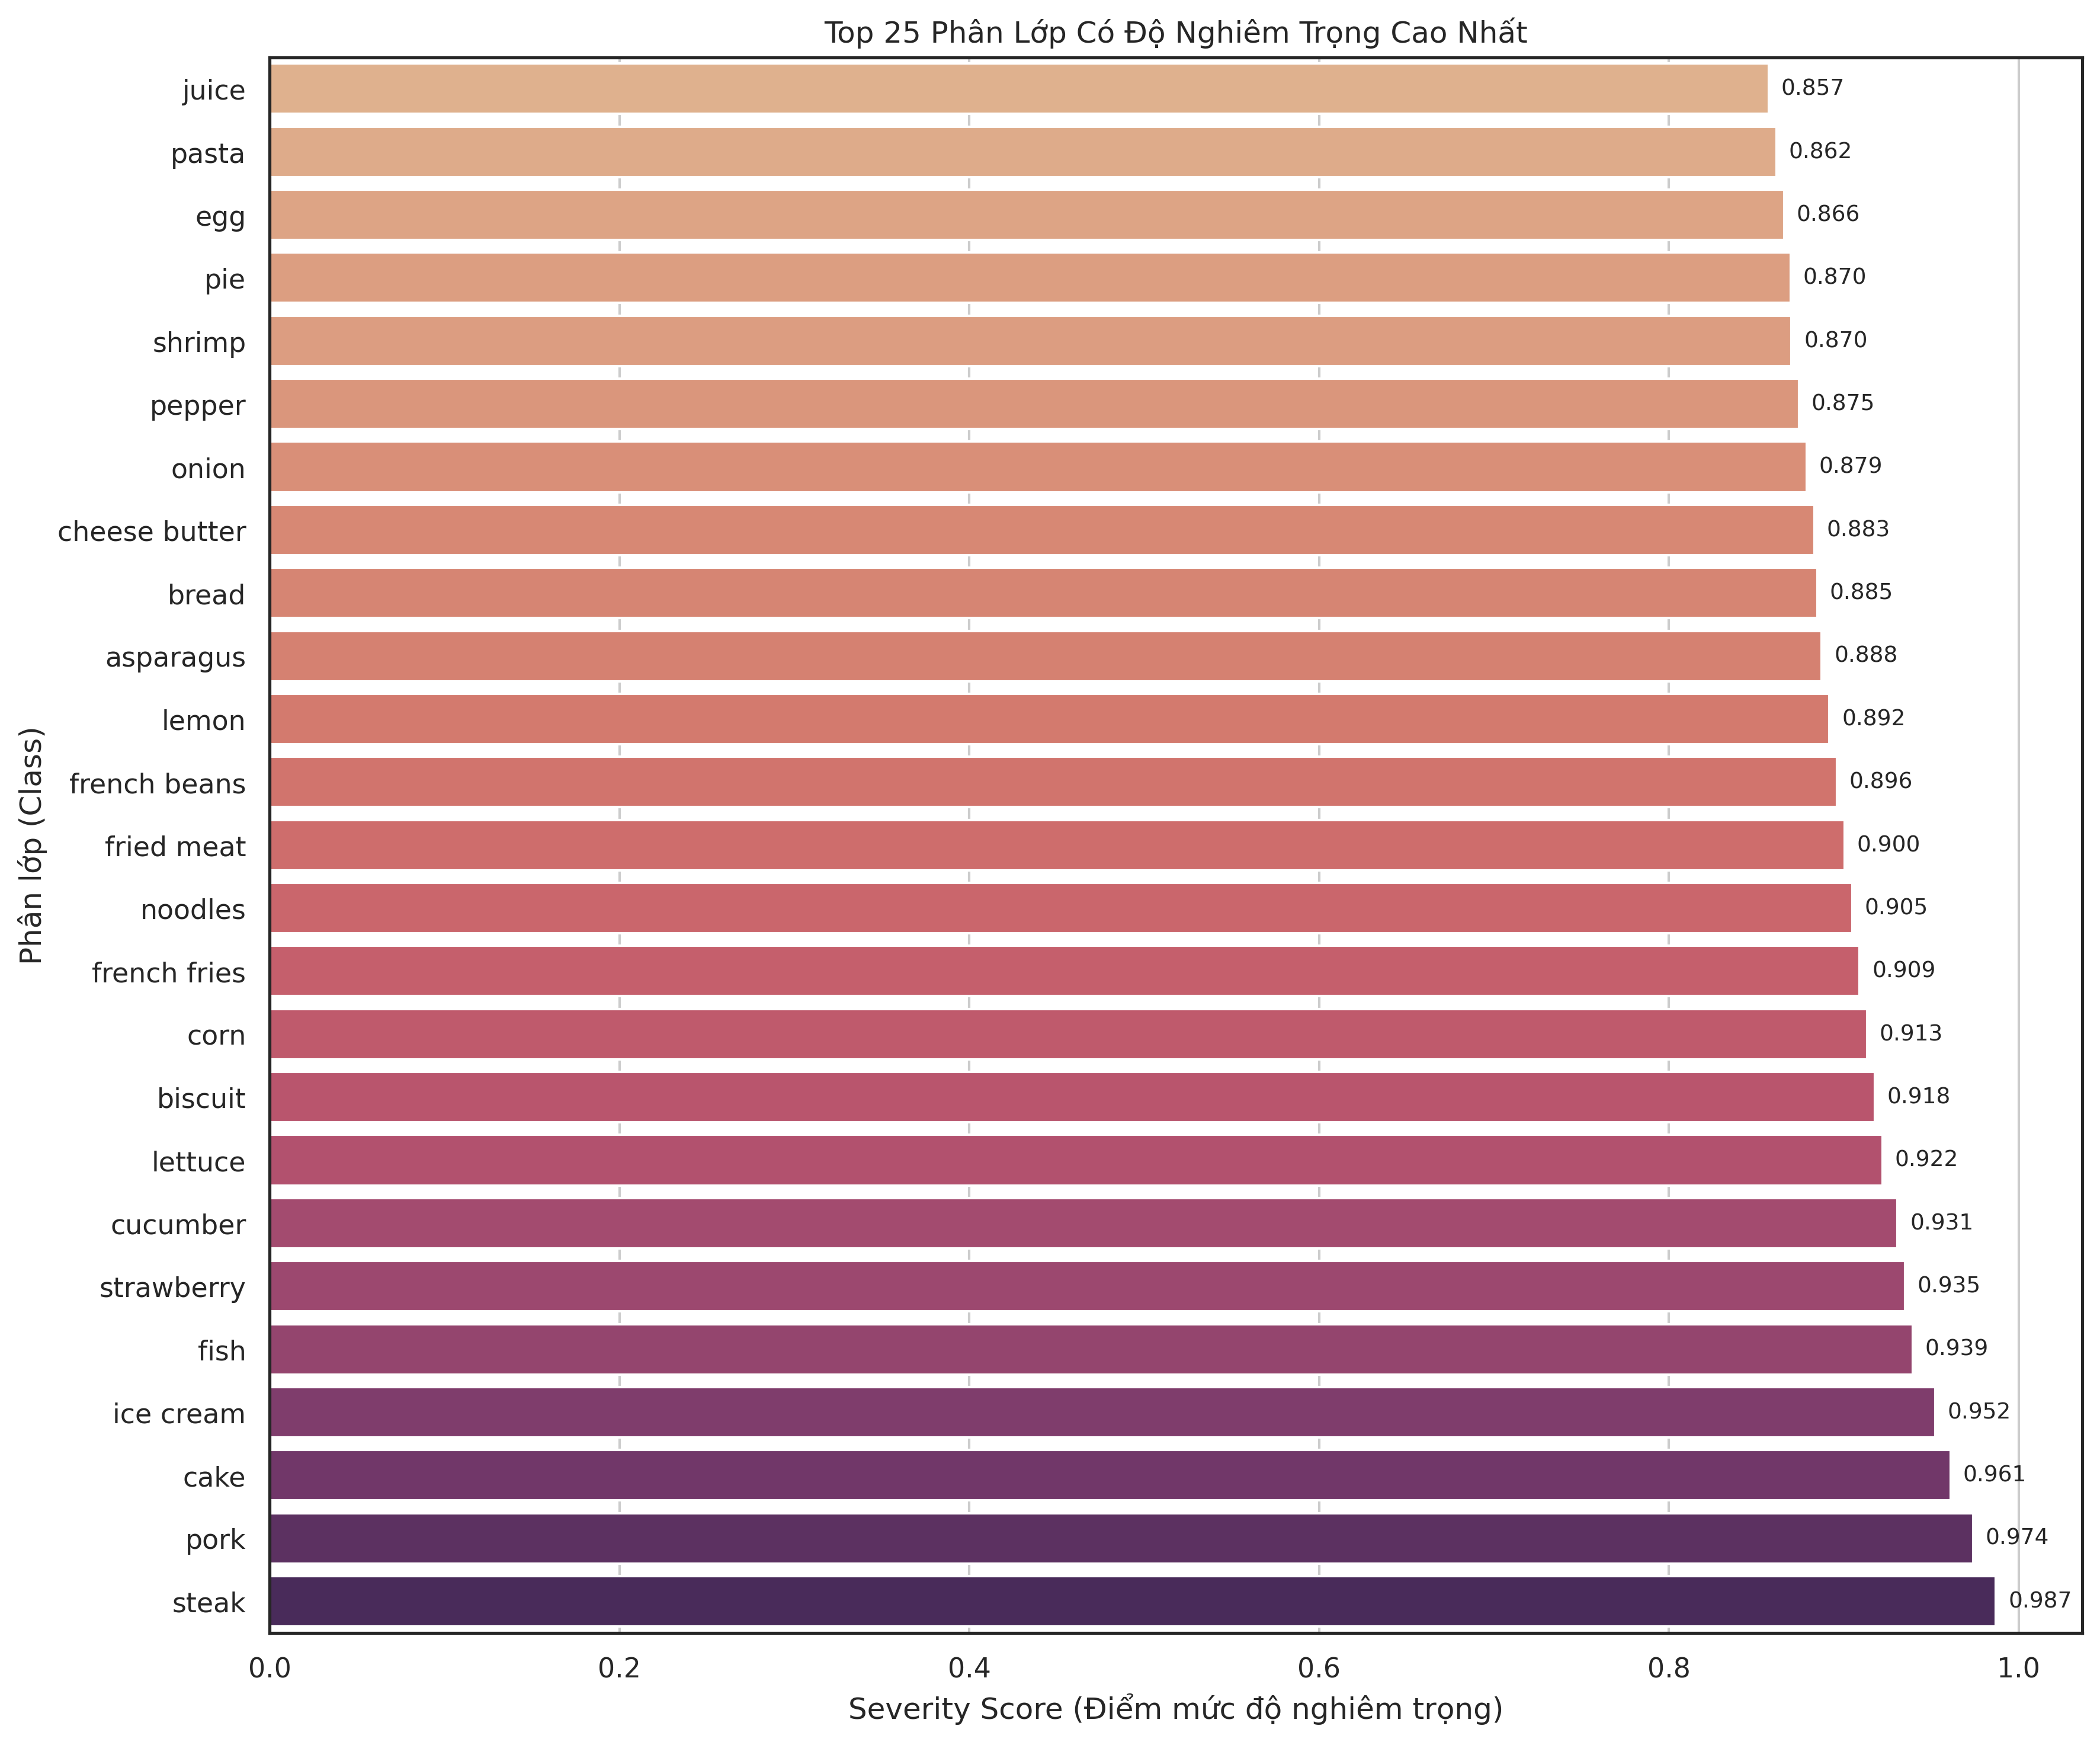
\includegraphics[width=\linewidth]{img/analyze/eval-model/01_class_severity_score_improved.png}
        \caption{Top lớp có điểm severity cao.}
        \label{fig:class_severity}
    \end{subfigure}
    \hfill
    \begin{subfigure}{0.49\linewidth}
        \centering
        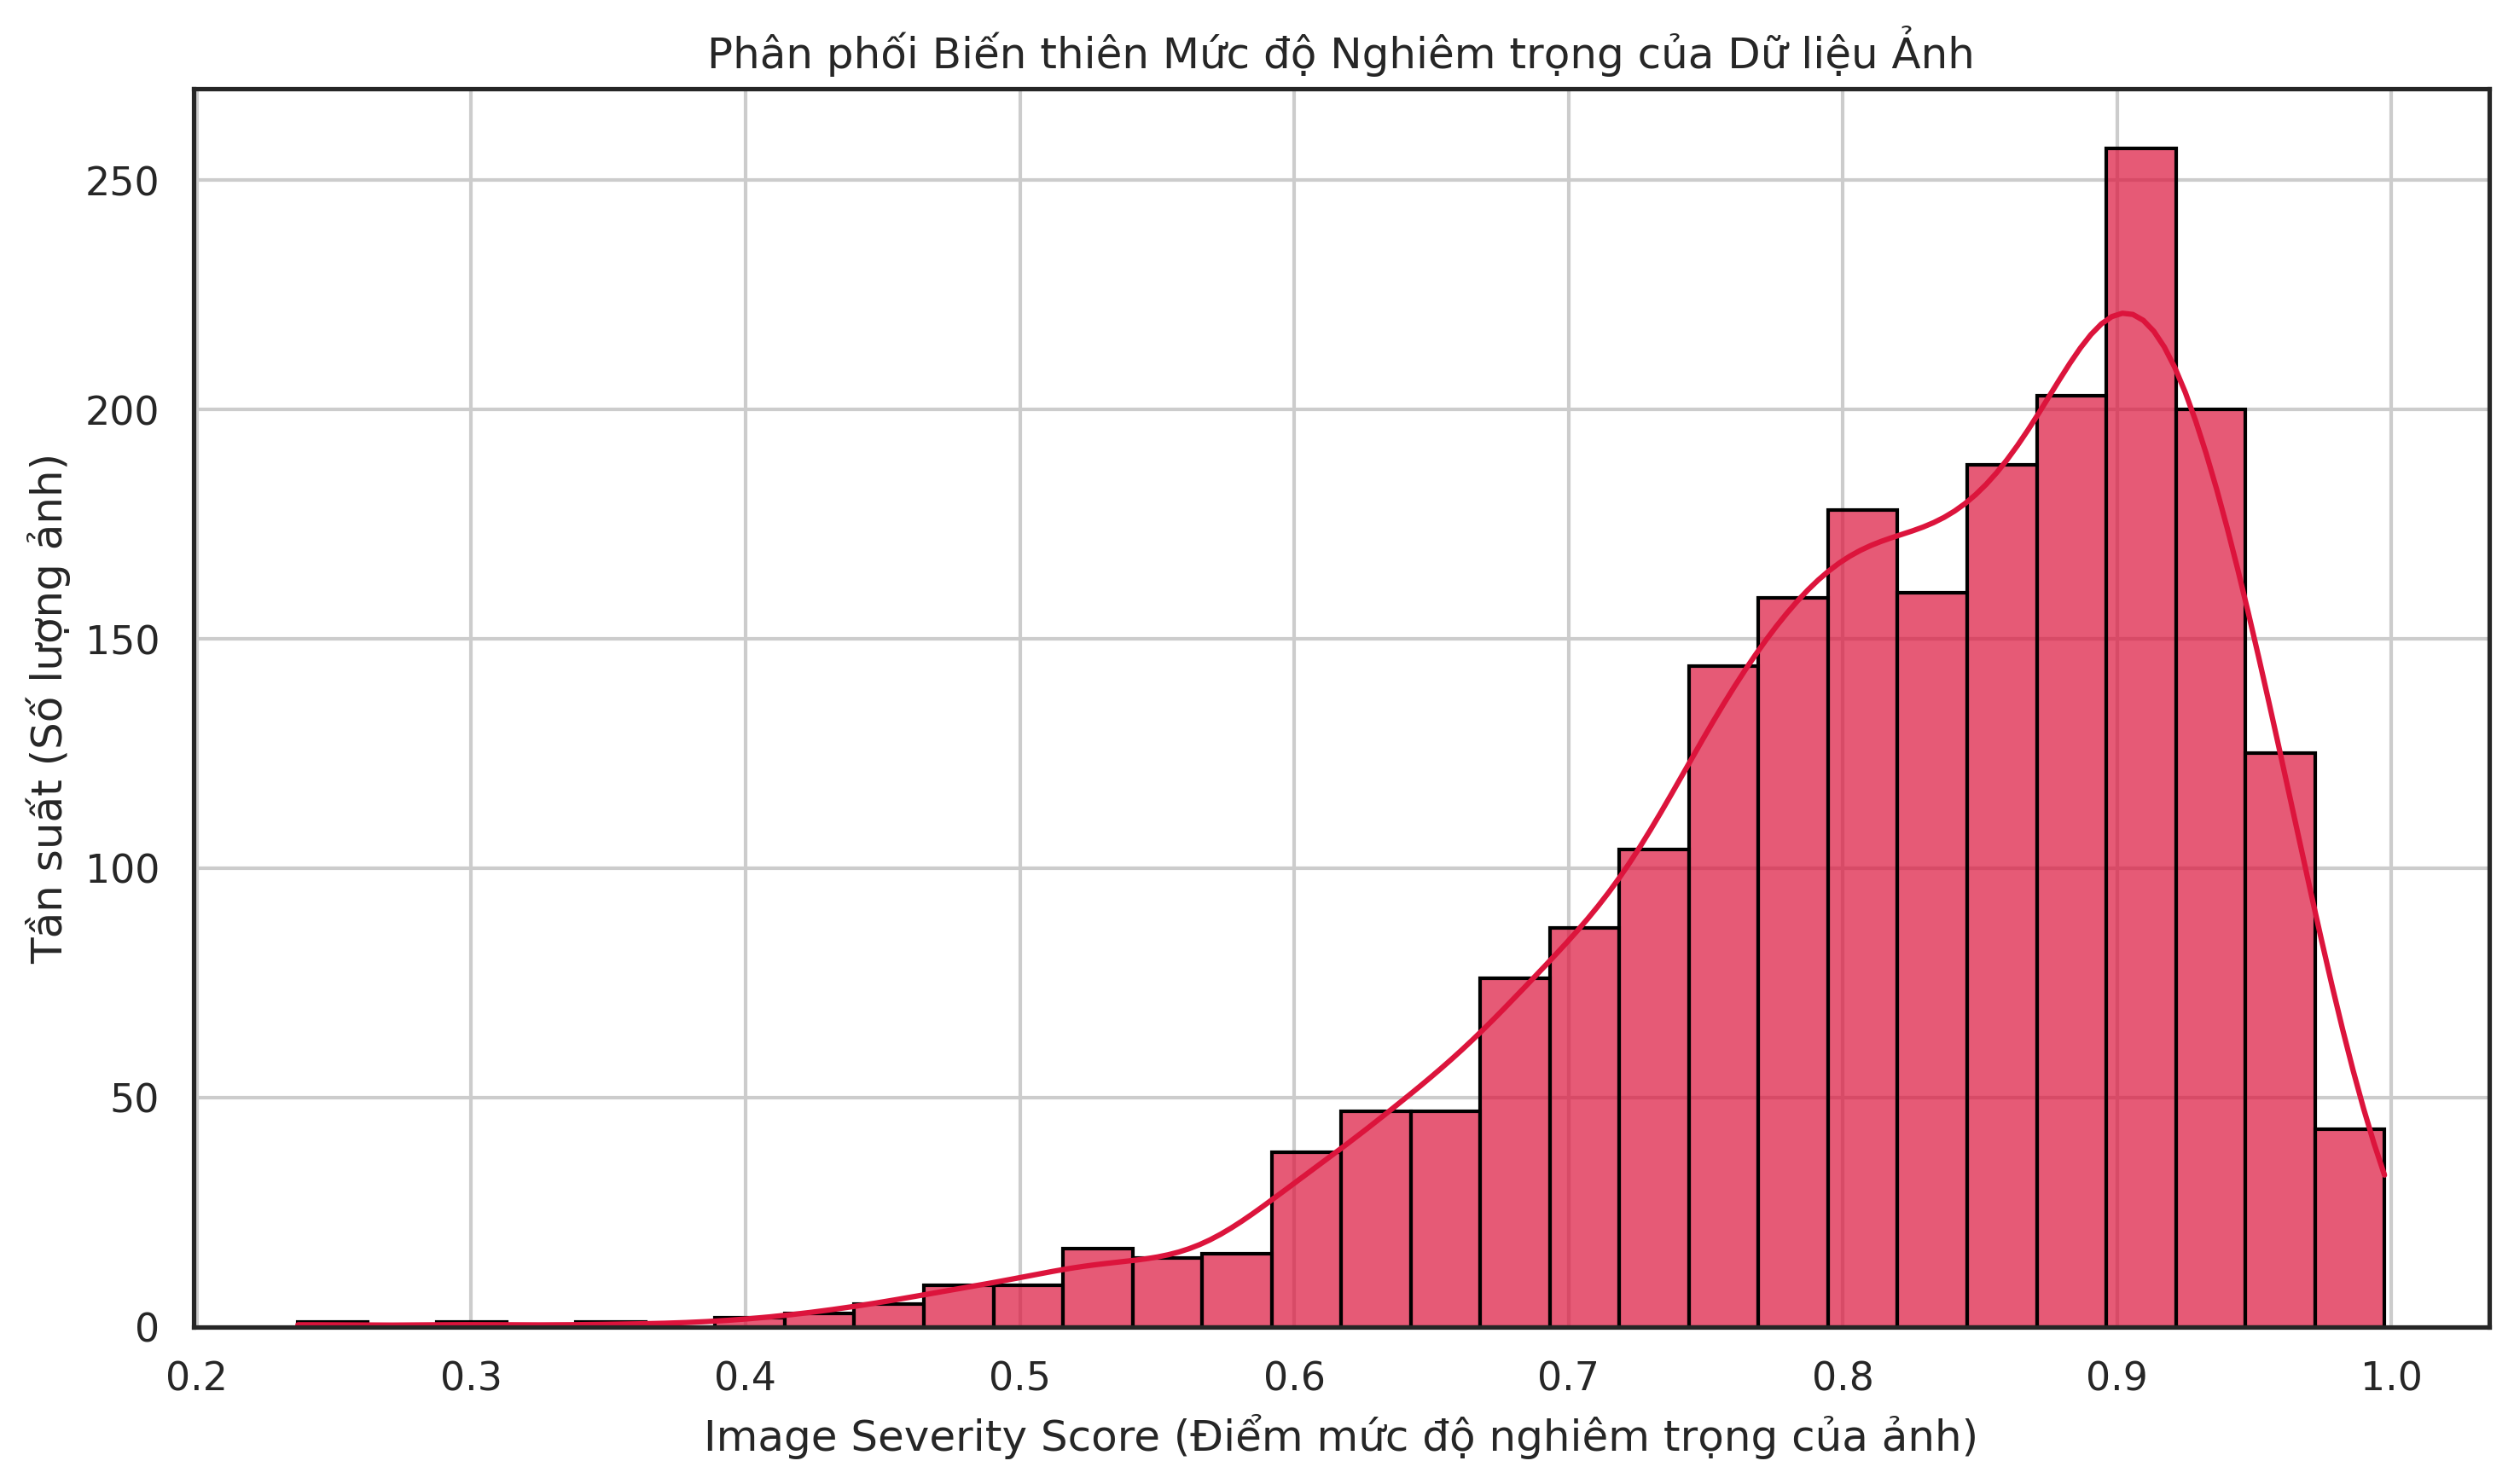
\includegraphics[width=\linewidth]{img/analyze/eval-model/02_image_severity_distribution_improved.png}
        \caption{Phân bố điểm độ nghiêm trọng ở mức ảnh.}
        \label{fig:image_severity_distribution}
    \end{subfigure}
    \caption{Nhóm phân tích mức độ khó dữ liệu theo lớp và theo ảnh (cụm 1--2).}
    \label{fig:pretrain_group_12}
\end{figure}

Phân bố lệch về phía giá trị cao có hai hàm ý quan trọng. Thứ nhất, nếu huấn luyện trực tiếp bằng lấy mẫu ngẫu nhiên, mô hình sẽ gặp ảnh khó với tần suất lớn ngay từ giai đoạn đầu, trong khi đặc trưng lớp chưa ổn định; điều này có thể làm tối ưu dao động và tăng nhầm lẫn giữa các lớp có texture gần nhau. Thứ hai, độ khó không chỉ nằm ở vài mẫu ngoại lệ mà là đặc tính phổ biến của toàn bộ dữ liệu. Vì vậy, hướng cải thiện không nên chỉ dừng ở tăng số epoch hoặc tăng backbone, mà cần xử lý trực tiếp các nguyên nhân gây khó như texture, boundary và quan hệ đồng xuất hiện giữa nguyên liệu.

\subsection{Cải tiến BiSeNet}
\label{subsec:proposed_bisenet_rtb}

Từ phân tích lỗi của baseline, BiSeNet còn hạn chế ở ba điểm chính: thiếu biểu diễn texture cục bộ, thiếu cơ chế mô hình hóa quan hệ giữa các lớp nguyên liệu, và chưa có giám sát trực tiếp tại vùng biên. Do đó, kiến trúc được đề xuất mở rộng BiSeNet theo ba thành phần: \textit{Texture-aware Branch}, \textit{Relation GNN Module} và \textit{Boundary-aware Supervision}. Các thành phần này được thiết kế theo dạng bổ sung nhẹ, không thay đổi cấu trúc hai nhánh cơ bản của BiSeNet.

\begin{figure}[H]
    \centering
    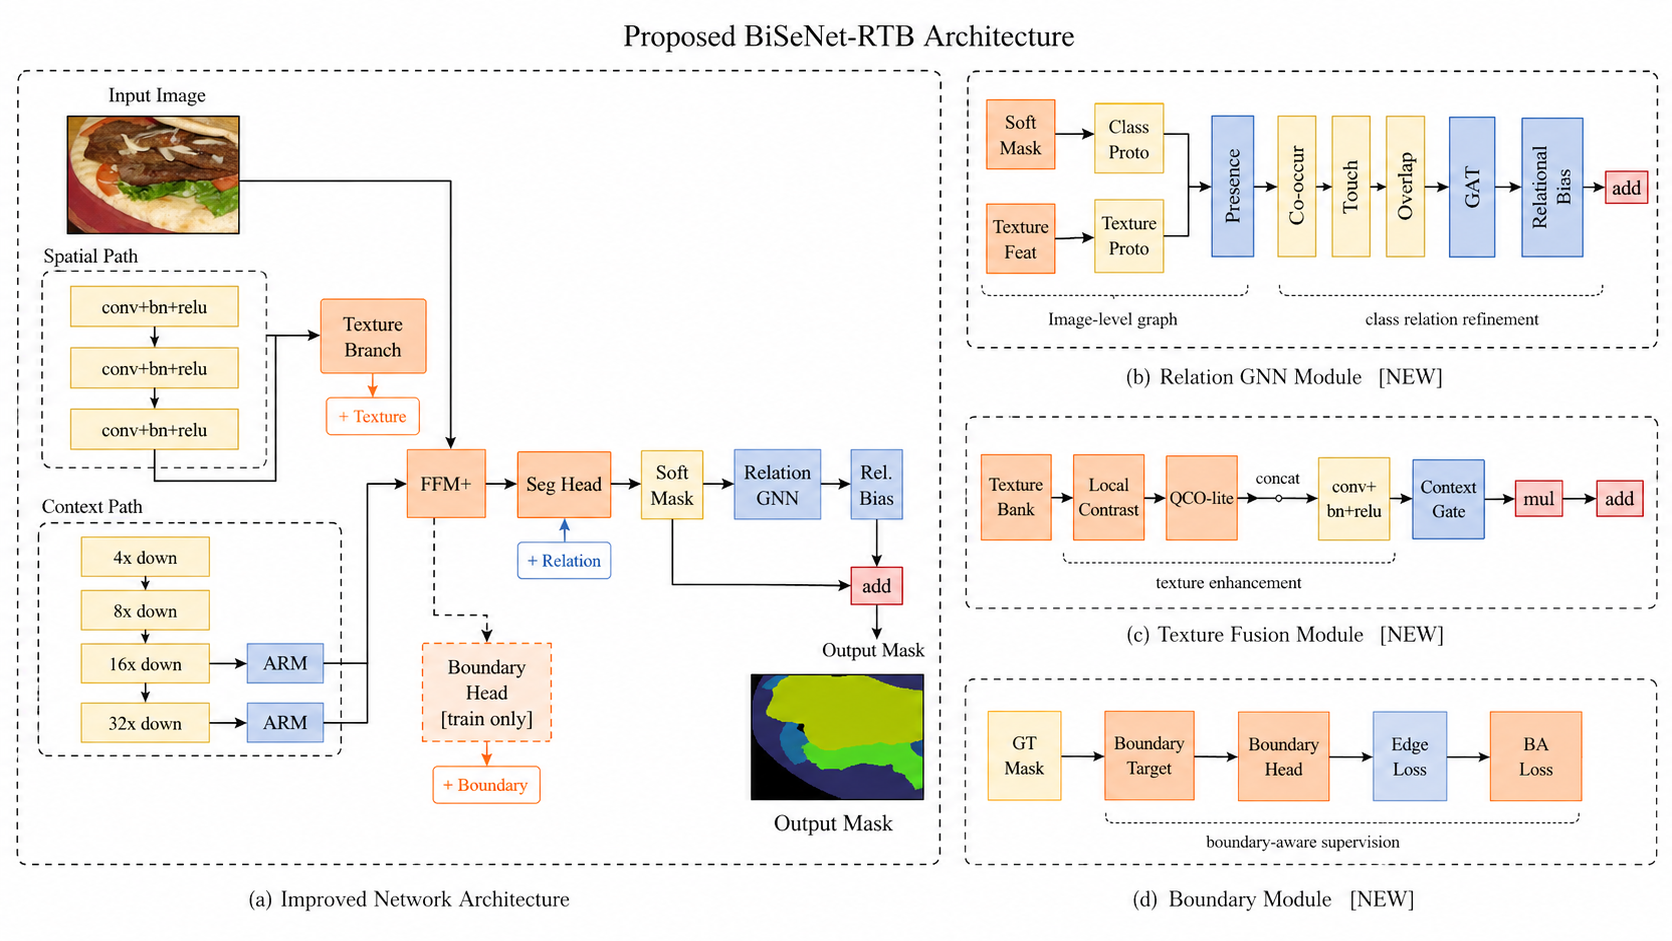
\includegraphics[width=\linewidth]{img/caitien/proposed_bisenet_architecture.png}
    \caption{Kiến trúc BiSeNet cải tiến với ba thành phần bổ sung: nhánh texture-aware, mô-đun Relation GNN và giám sát biên.}
    \label{fig:improved_bisenet_rtb}
\end{figure}

\subsubsection{Texture-aware Branch}

Spatial Path của BiSeNet giữ lại đặc trưng độ phân giải cao, nhưng chưa có cơ chế chuyên biệt để khai thác texture. Vì vậy, một nhánh texture nhẹ được thêm vào từ đặc trưng không gian $F_{sp}$. Nhánh này trích xuất các tín hiệu cục bộ như cạnh nhỏ, độ tương phản vùng lân cận và cấu trúc bề mặt.

Gọi đặc trưng texture là $T$, quá trình tăng cường Spatial Path được viết $ T = \phi_{\text{tex}}(F_{sp})$ và $F_{sp}^{tex} = F_{sp} + \psi([F_{sp}, T])$

trong đó $\phi_{\text{tex}}$ là nhánh trích xuất texture, $\psi$ là phép biến đổi tích chập nhẹ, và $[\cdot,\cdot]$ là phép nối kênh. Đặc trưng $F_{sp}^{tex}$ sau đó được đưa vào Feature Fusion Module để hợp nhất với đặc trưng ngữ cảnh từ Context Path.

Mục tiêu của thành phần này là tăng khả năng phân biệt các lớp có màu sắc và hình thái gần nhau nhưng khác nhau ở texture bề mặt, ví dụ các nhóm thịt, bánh, sốt hoặc rau đã qua chế biến.

\subsubsection{Relation GNN Module}

Các lỗi nhầm lẫn của baseline cho thấy một số lớp có xu hướng bị dự đoán quá mức, đồng thời nhiều cặp lớp thường bị nhầm do đồng xuất hiện hoặc tiếp xúc trong cùng ảnh. Để mô hình hóa quan hệ này, một đồ thị lớp được xây dựng trên không gian nhãn.

Sau khi segmentation head sinh logits sơ bộ $Y \in \mathbb{R}^{K \times H \times W}$, xác suất mềm của lớp $i$ tại pixel $u$ được tính bởi $q_i(u) = \mathrm{softmax}(Y)_i(u)$.

Từ đó, class prototype của lớp $i$ được lấy bằng pooling có trọng số theo soft mask:
\[
f_i =
\frac{\sum_{u} q_i(u)F(u)}
{\sum_{u}q_i(u)+\epsilon},
\]

trong đó $F$ là đặc trưng sau fusion. Nếu sử dụng thêm texture feature $T$, texture prototype được tính tương tự:
\[
\tau_i =
\frac{\sum_{u} q_i(u)T(u)}
{\sum_{u}q_i(u)+\epsilon}.
\]

Node feature của lớp $i$ được định nghĩa: $x_i = [W_f f_i \; || \; W_t \tau_i \; || \; a_i]$,

với $a_i = \frac{1}{HW}\sum_u q_i(u)$ là diện tích mềm của lớp $i$, $W_f$ và $W_t$ là các phép chiếu tuyến tính.

Ma trận cạnh $A$ được xây dựng từ thống kê nội bộ của tập huấn luyện, gồm xác suất đồng xuất hiện, mức độ tiếp xúc biên và mức độ chồng lấp mềm: $A = \mathrm{row\_norm}\!\left(\alpha A_{\text{cooc}} + \beta A_{\text{touch}} + \gamma A_{\text{overlap}}\right)$,

trong đó $A_{\text{cooc}}$ biểu diễn quan hệ đồng xuất hiện, $A_{\text{touch}}$ biểu diễn quan hệ tiếp xúc biên, và $A_{\text{overlap}}$ biểu diễn mức chồng lấp mềm sau dilation.

GNN cập nhật biểu diễn lớp theo dạng:
\[
h_i^{(l+1)} = \sigma\!\left(\sum_{j \in \mathcal{N}(i)} A_{ij} W^{(l)} h_j^{(l)}\right).
\]

Sau $L$ lớp GNN, biểu diễn quan hệ $h_i^{(L)}$ được dùng để sinh relational bias $b_i = w_b^\top h_i^{(L)}$. Logits cuối cùng được hiệu chỉnh bởi $Y'_i(u) = Y_i(u) + \eta b_i$.

Thành phần này nhằm giảm các lỗi có cấu trúc, đặc biệt là hiện tượng sink class và các nhầm lẫn giữa các lớp thường đồng xuất hiện trong ảnh món ăn.

\subsubsection{Boundary-aware Supervision}

BiSeNet gốc không có nhánh giám sát biên tường minh, trong khi lỗi mIoU thường xuất hiện ở vùng chuyển tiếp giữa các nguyên liệu. Do đó, một Boundary Head được thêm vào trong giai đoạn huấn luyện để tăng ràng buộc tại vùng biên.

Từ ground-truth mask $S$, bản đồ biên $B$ được sinh bằng phép morphological gradient: $B = \mathrm{Dilate}(S) - \mathrm{Erode}(S)$.

Boundary Head nhận đặc trưng $F_{sp}^{tex}$ và dự đoán bản đồ biên $\hat{B} = \phi_{\text{bd}}(F_{sp}^{tex})$.

Loss biên được định nghĩa bằng weighted binary cross-entropy kết hợp Dice loss: 
\[
L_{\text{edge}}
=
\mathrm{WBCE}(\hat{B}, B)
+
\lambda_d L_{\text{Dice}}(\hat{B}, B).
\]

Ngoài ra, để nhấn mạnh lỗi semantic tại vùng biên, một boundary-aware loss được áp dụng trên tập pixel biên $\Omega_b$: $L_{\text{ba}} = -\frac{1}{|\Omega_b|}\sum_{u \in \Omega_b}\log p_{S(u)}(u)$, trong đó $p_{S(u)}(u)$ là xác suất dự đoán của lớp đúng tại pixel $u$.

Boundary Head chỉ được sử dụng để tăng giám sát trong huấn luyện. Khi suy luận, nhánh này có thể được loại bỏ để giữ chi phí tính toán gần với baseline.

\subsubsection{Hàm mất mát tổng}

Mô hình được huấn luyện bằng tổ hợp loss: $L_{\text{total}} = L_{\text{seg}} + \lambda_{\text{edge}} L_{\text{edge}} + \lambda_{\text{ba}} L_{\text{ba}} + \lambda_{\text{rel}} L_{\text{rel}}$.

Trong đó $L_{\text{seg}}$ là loss phân đoạn chính, $L_{\text{edge}}$ giám sát bản đồ biên, $L_{\text{ba}}$ tăng trọng số lỗi tại vùng biên, và $L_{\text{rel}}$ là loss phụ cho dự đoán hiện diện lớp hoặc ràng buộc quan hệ lớp nếu được sử dụng.

\begin{table}[H]
\centering
\caption{Vai trò của các thành phần cải tiến trong BiSeNet đề xuất}
\label{tab:proposed_components}
\begin{tabular}{p{0.2\linewidth}p{0.28\linewidth}p{0.25\linewidth}}
\toprule
\textbf{Thành phần} & \textbf{Mục tiêu} & \textbf{Lỗi nhắm đến} \\
\midrule
Texture-aware Branch 
& Bổ sung đặc trưng texture cục bộ vào Spatial Path 
& Nhầm lẫn giữa các lớp có bề mặt giống nhau \\
\midrule
Relation GNN 
& Mô hình hóa quan hệ đồng xuất hiện, tiếp xúc và chồng lấp giữa lớp 
& Sink class, nhầm lẫn có cấu trúc \\
\midrule
Boundary-aware Supervision 
& Tăng giám sát tại vùng biên giữa các nguyên liệu 
& Mask tràn biên, dính lớp, bỏ sót vùng nhỏ \\
\bottomrule
\end{tabular}
\end{table}

\subsection{Kết quả}

Hình~\ref{fig:gnn-prior-analysis} trình bày prior đồ thị được xây dựng từ thống kê đồng xuất hiện và tiếp xúc biên giữa các lớp nguyên liệu. Đồ thị các cạnh mạnh cho thấy một số lớp \textit{head} như \texttt{bread}, \texttt{chicken duck}, \texttt{tomato}, \texttt{potato} và \texttt{broccoli} đóng vai trò nút liên kết với nhiều lớp \textit{medium}; điều này phù hợp với giả thuyết rằng lỗi phân đoạn không độc lập theo từng lớp mà có cấu trúc theo ngữ cảnh món ăn. Heatmap thành phần đồng xuất hiện cũng cho thấy các cụm quan hệ có cường độ cao, cung cấp tín hiệu prior để Relation GNN điều chỉnh logits theo các lớp thường xuất hiện cùng nhau hoặc nằm sát nhau trên ảnh.

\begin{figure}[H]
    \centering
    \begin{subfigure}{0.49\linewidth}
        \centering
        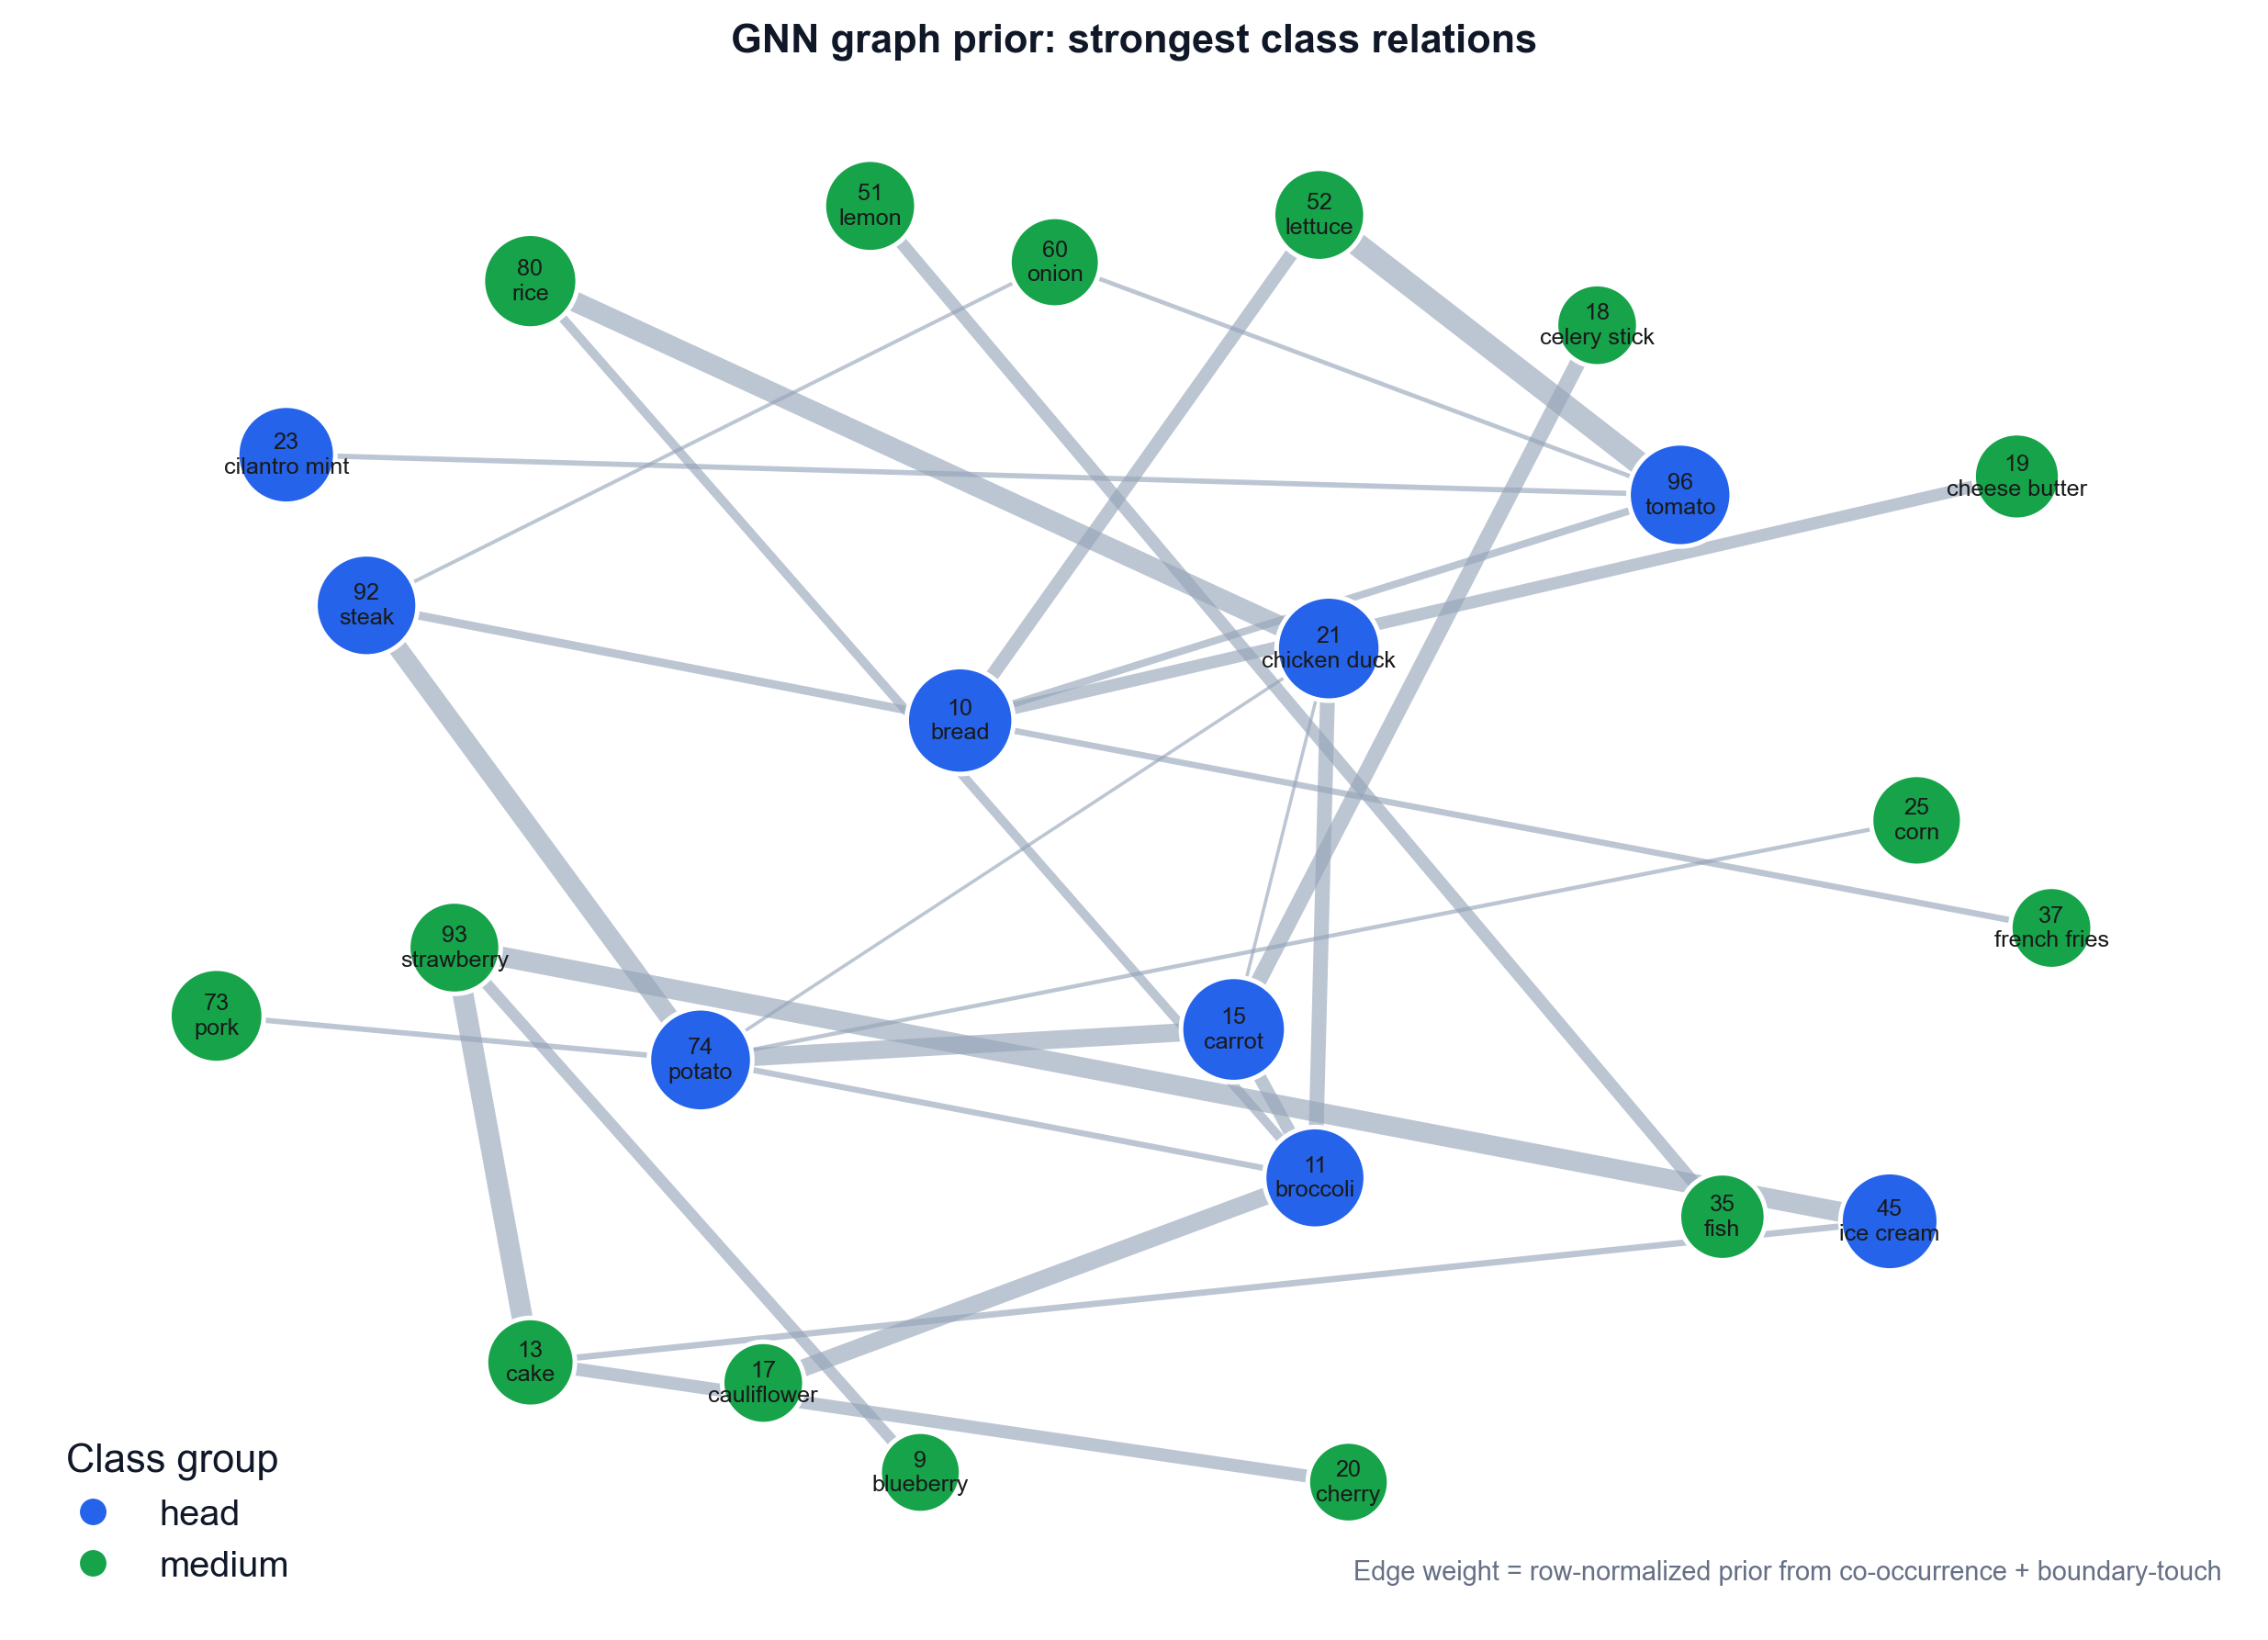
\includegraphics[width=\linewidth]{img/caitien/plot/08_gnn_prior_top_edges_network.png}
        \caption{Các quan hệ lớp mạnh nhất trong prior GNN.}
        \label{fig:gnn-prior-network}
    \end{subfigure}
    \hfill
    \begin{subfigure}{0.49\linewidth}
        \centering
        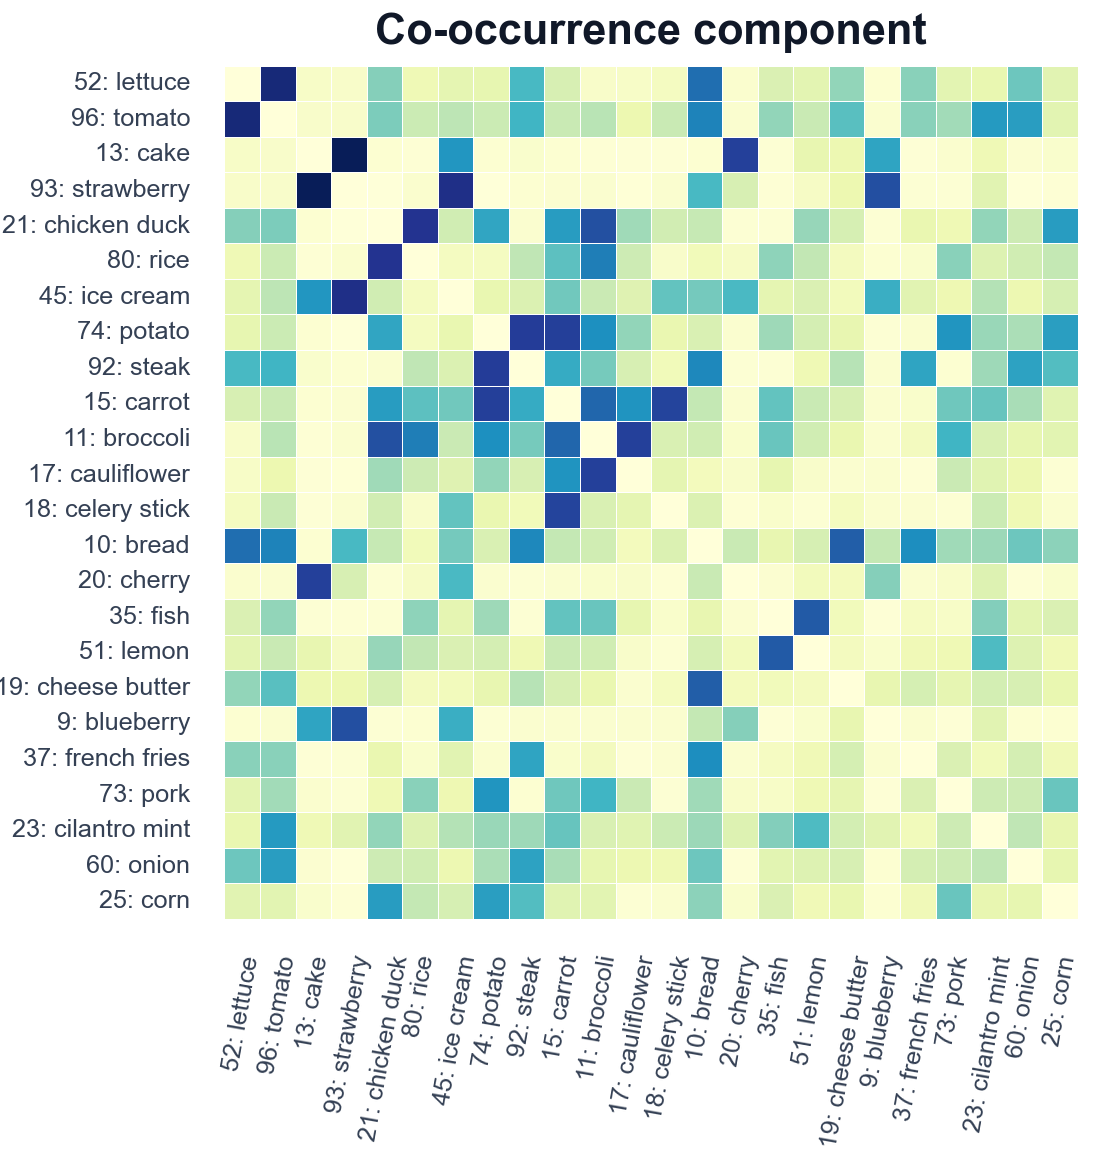
\includegraphics[width=\linewidth]{img/caitien/plot/09_gnn_prior_components_heatmap.png}
        \caption{Heatmap thành phần đồng xuất hiện.}
        \label{fig:gnn-prior-heatmap}
    \end{subfigure}
    \caption{Phân tích prior đồ thị lớp dùng cho Relation GNN.}
    \label{fig:gnn-prior-analysis}
\end{figure}

Hình~\ref{fig:rtb-training-curves} cho thấy mô hình RTB/GNN hội tụ ổn định trong quá trình huấn luyện. Loss huấn luyện giảm đều từ giai đoạn đầu đến cuối, trong khi validation loss giảm nhanh và ổn định quanh vùng thấp sau khoảng 60 epoch; checkpoint tốt nhất theo validation loss nằm ở epoch 129. Các chỉ số validation tăng cùng chiều với quá trình giảm loss, trong đó \texttt{mIoU} và \texttt{mAcc} đạt tốt nhất ở epoch 141, còn \texttt{aAcc} đạt tốt nhất ở epoch 129. Xu hướng này cho thấy các thành phần texture, boundary và prior GNN giúp mô hình cải thiện không chỉ độ chính xác toàn cục mà còn cả khả năng phân biệt trung bình theo lớp.

\begin{figure}[H]
    \centering
    \begin{subfigure}{0.49\linewidth}
        \centering
        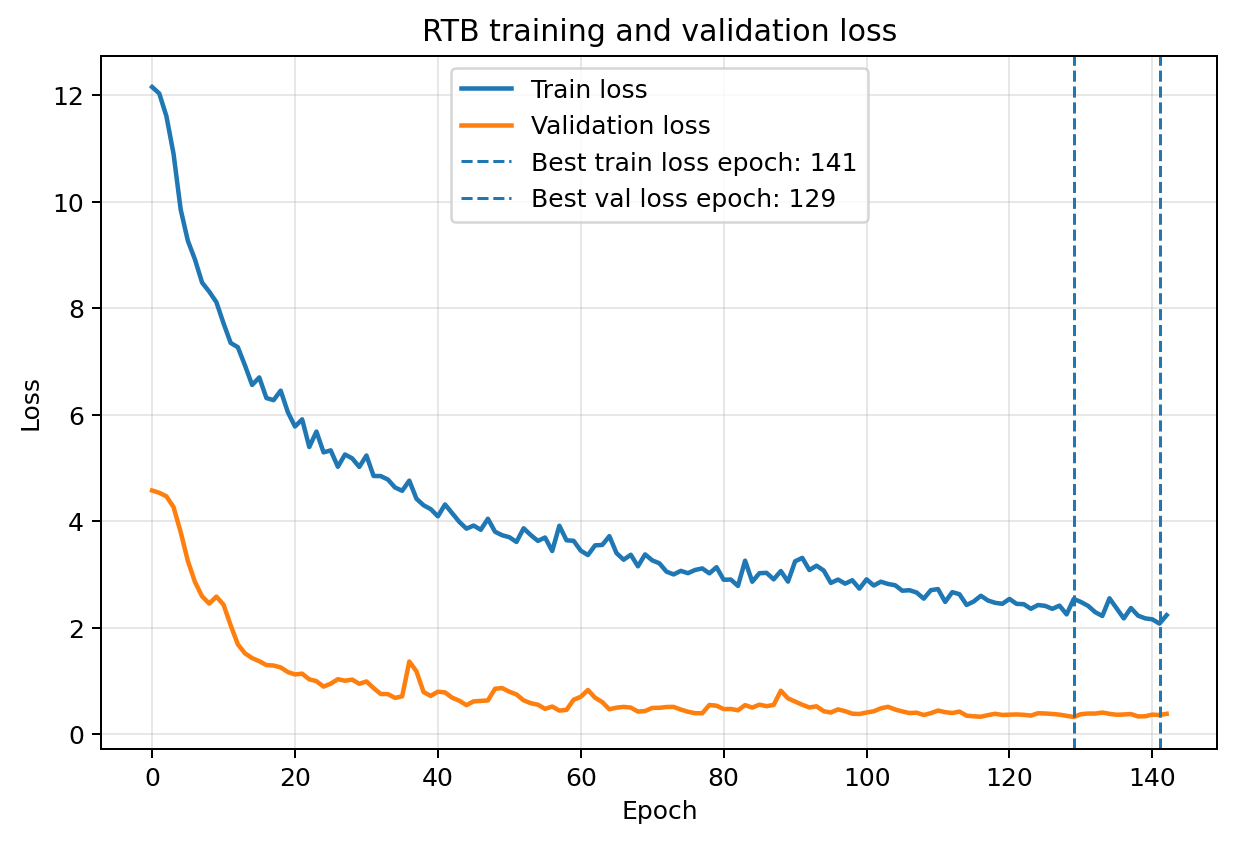
\includegraphics[width=\linewidth]{img/caitien/plot/rtb_best_loss.png}
        \caption{Train loss và validation loss.}
        \label{fig:rtb-best-loss}
    \end{subfigure}
    \hfill
    \begin{subfigure}{0.49\linewidth}
        \centering
        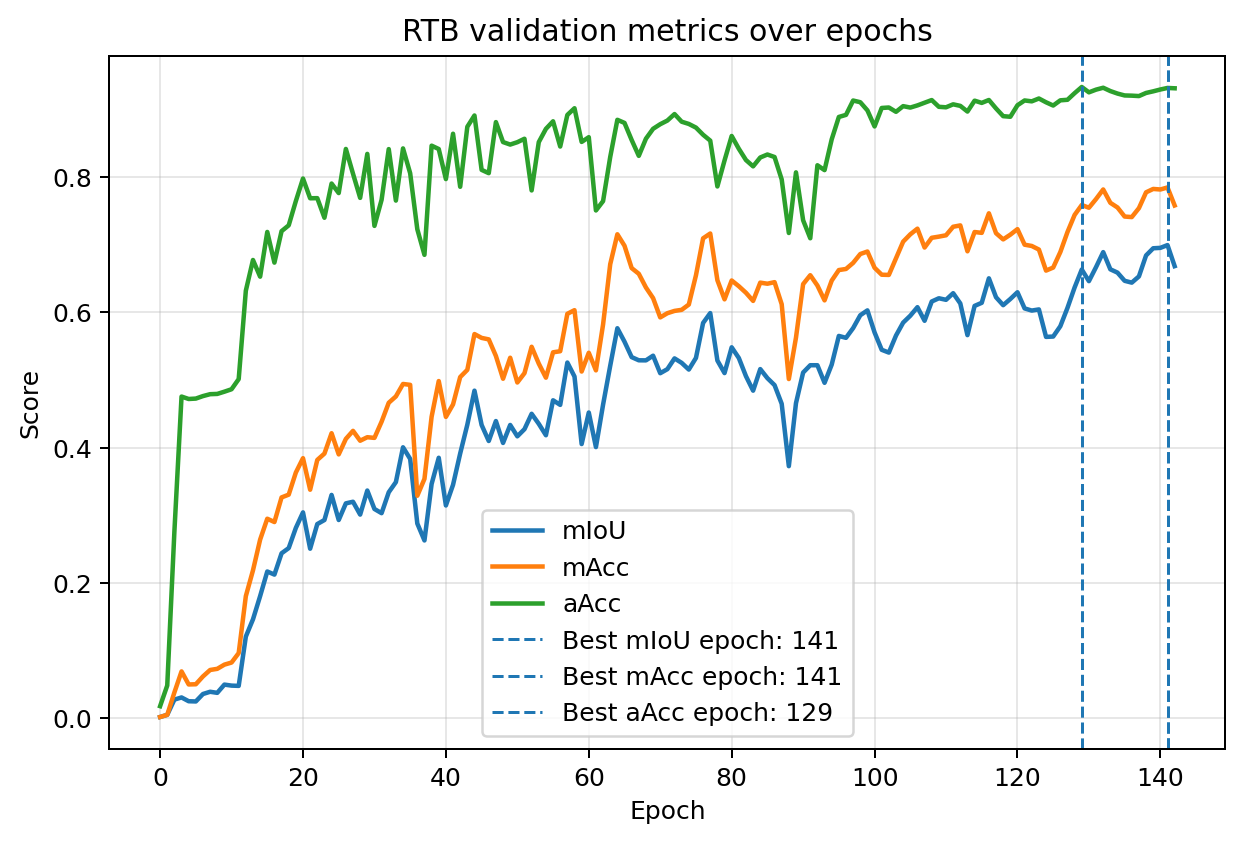
\includegraphics[width=\linewidth]{img/caitien/plot/rtb_best_metrics.png}
        \caption{Các chỉ số validation theo epoch.}
        \label{fig:rtb-best-metrics}
    \end{subfigure}
    \caption{Diễn biến huấn luyện và đánh giá validation của mô hình RTB/GNN.}
    \label{fig:rtb-training-curves}
\end{figure}

Hình~\ref{fig:rtb-comparison-presence} so sánh checkpoint tốt nhất của mô hình đề xuất với các baseline và phân tích lỗi hiện diện lớp. Ở checkpoint tốt nhất, RTB/GNN đạt \texttt{mIoU} $59.9\%$, \texttt{mAcc} $71.7\%$ và \texttt{aAcc} $85.4\%$, cao hơn rõ rệt so với CCNet và BiSeNetV1 trên cả ba chỉ số. Phân tích presence cho thấy mô hình ban đầu chủ yếu tạo lỗi dương giả, trong khi các checkpoint sau giảm mạnh lỗi này; checkpoint tốt nhất theo presence đạt độ chính xác hiện diện $100\%$, còn checkpoint tốt nhất theo \texttt{mIoU} đạt $87.5\%$. Điều này cho thấy prior GNN và các ràng buộc bổ sung giúp mô hình kiểm soát tốt hơn việc dự đoán lớp có/không xuất hiện, qua đó giảm hiện tượng dự đoán lan sang các lớp không có trong ảnh.

\begin{figure}[H]
    \centering
    \begin{subfigure}{0.49\linewidth}
        \centering
        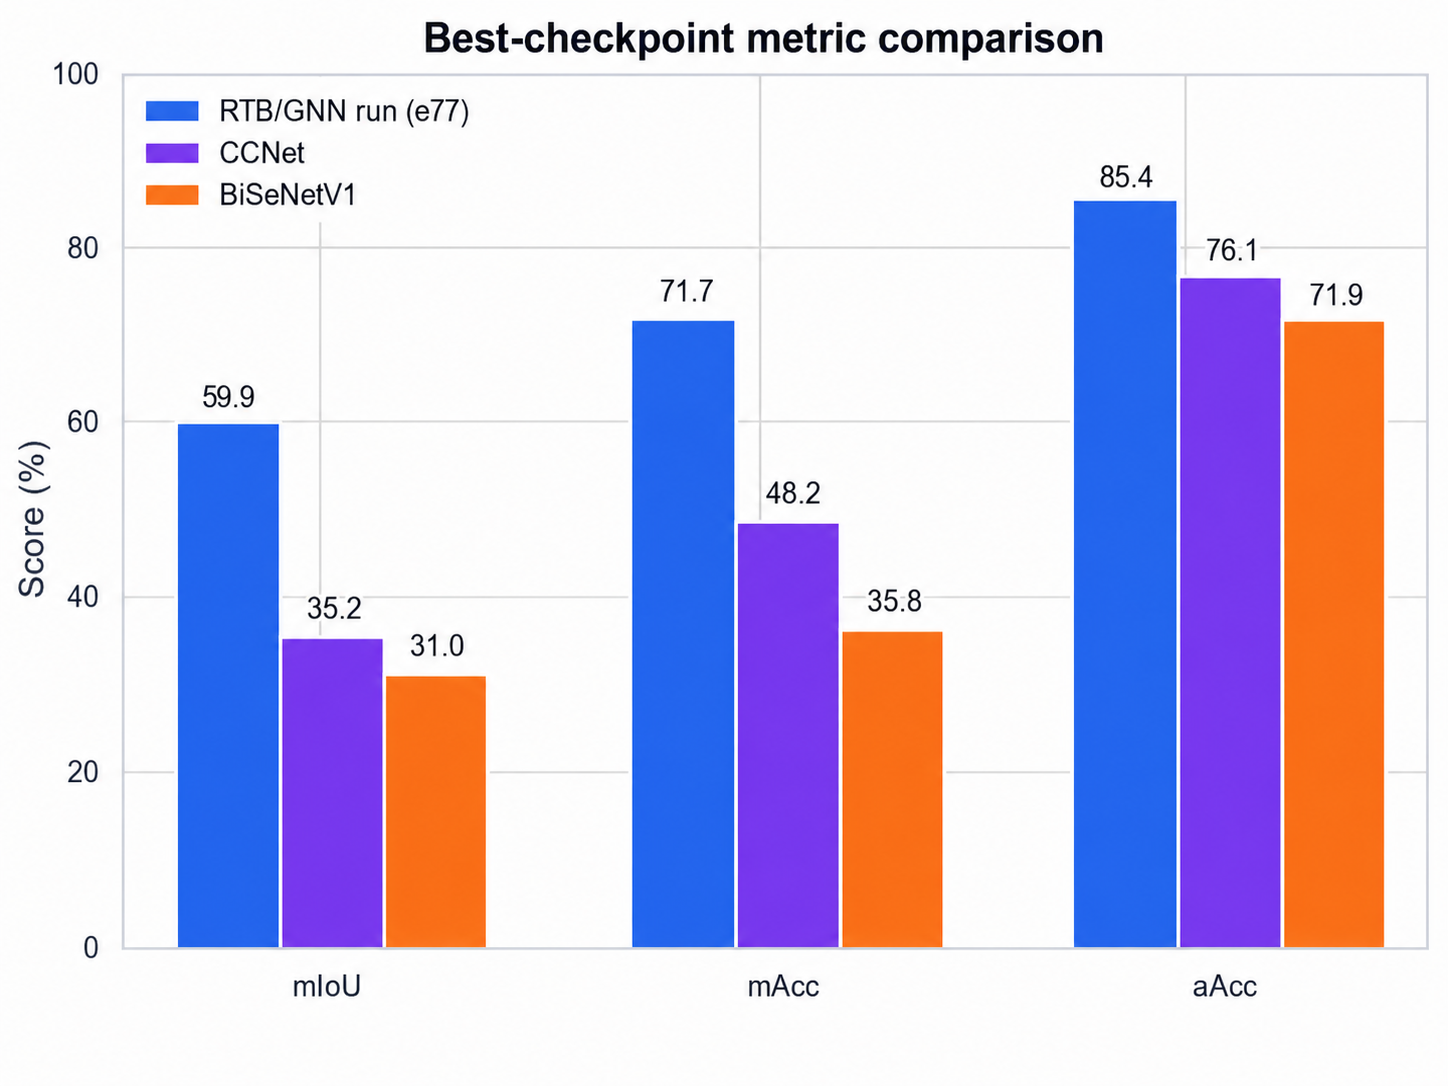
\includegraphics[width=\linewidth]{img/caitien/plot/best-comparison-metric.png}
        \caption{So sánh chỉ số với các baseline.}
        \label{fig:rtb-best-comparison}
    \end{subfigure}
    \hfill
    \begin{subfigure}{0.49\linewidth}
        \centering
        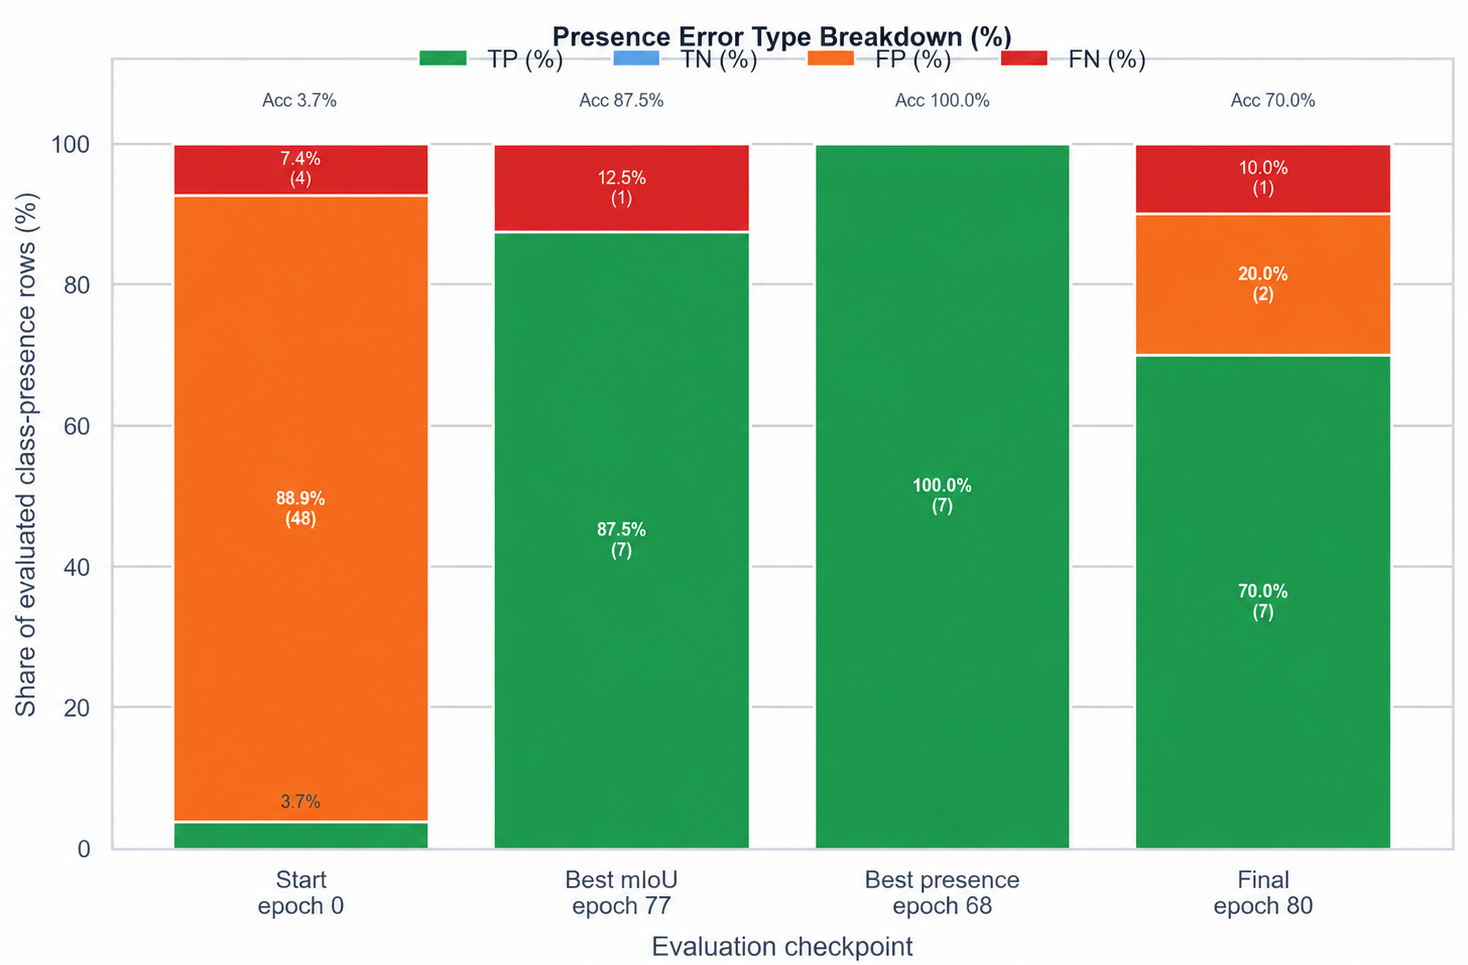
\includegraphics[width=\linewidth]{img/caitien/plot/presence error.png}
        \caption{Phân tích lỗi hiện diện lớp.}
        \label{fig:rtb-presence-error}
    \end{subfigure}
    \caption{So sánh hiệu năng và phân tích lỗi presence của mô hình RTB/GNN.}
    \label{fig:rtb-comparison-presence}
\end{figure}

